\documentclass{article}
\usepackage[utf8]{inputenc}

\title{Causal Graphical Models }
% \author{David Johnston}

\usepackage[mathscr]{euscript}
\usepackage{natbib}
\usepackage{graphicx}
\usepackage {tikz}
\usetikzlibrary {positioning}
\usepackage[a4paper, margin=0.7in]{geometry}
\setlength{\parskip}{1em}
\setlength{\parindent}{0em}
\usepackage{amsthm}
\usepackage{amsmath}
\usepackage{amssymb}
\usepackage{dsfont}
\usepackage{hyperref}

\theoremstyle{definition}
\newtheorem{question}{Question}[section]
\newtheorem{definition}{Definition}[section]
\newtheorem{example}{Example}[section]
 
\theoremstyle{remark}
\newtheorem*{remark}{Remark}

 
\newtheorem{theorem}{Theorem}[section]
\newtheorem{corollary}{Corollary}[theorem]
\newtheorem{lemma}[theorem]{Lemma}

\setcounter{secnumdepth}{6}

\newcommand{\NC}[2]{\ensuremath{{#1}\not\to{#2}}}
\newcommand{\CI}{\mathrel{\text{\scalebox{1.07}{$\perp\mkern-10mu\perp$}}}}

\begin{document}

\maketitle

\tableofcontents
\newpage


\section{Philosophical Preliminaries}

Causality is an imprecise concept for which various mathematical formalisations have been proposed. There is ongoing debate as to whether the mathematical formalisations adequately capture the concept. The approach here is to agnostic on the nature of causes and instead focuses on the efficacy of the mathematical formalisms in addressing particular types of query. We will call the formalisms causal models and the queries causal queries, but our relationship to the metaphysics of causality is as an inspiration for potentially useful methods rather than a true form we seek to emulate.

\section{Graphical Models}


\begin{definition}[Directed Acyclic Graph]
A Directed Acyclic Graph (DAG) $G$ is a set of vertices and directed edges $(V,E)$. A directed edge $E$ is an ordered pair of vertices $V_1$ and $V_2$, is represented by $V_1 \to V_2$ and identifies $V_1$ as a parent of $V_2$ and $V_2$ as a child of $V_1$. We say the head of $E$ points to $V_2$ and the tail points to $V_1$.
\end{definition}

\begin{definition}[Paths and Directed Paths:]
A path $p$ consists of a sequence of nodes $\mathcal{V}=\{V_i:1\leq i \leq n\}$, $n\in\mathbb{N}$ along with a sequence of edges $\mathcal{E}=\{E_i:1\leq i \leq n-1\}$. The edge $E_i$ connects nodes $V_i$ and $V_{i+1}$, no edge appears in $\mathcal{E}$ more than once and no vertex appears in $\mathcal{V}$ more than once.

A directed path is a path from $V_i$ to $V_j$ such that every edge $E_k$ is oriented from $V_k$ to $V_{k+1}$.
\end{definition}

\begin{definition}[Descendants and Ancestors]\label{def:descendants_and_ancestors}
A descendant of $V_i$ in $G$ is a child of $V_i$ or the child of a descendant of $V_i$. Equivalently, $V_j$ is a descendant of $V_i$ iff there is a directed path from $V_i$ to $V_j$.

An ancestor of $V_i$ in $G$ is a parent of $V_i$ or a parent of an ancestor of $V_i$. Equivalently, $V_j$ is an ancestor of $V_i$ iff there is a directed path from $V_j$ to $V_i$.
\end{definition}

\begin{definition}[Head-to-head node]
A head to head or collider node $V_{h}$ in a path $p$ is a node where the two adjacent edges $E_i$ and $E_{i+1}$ in $p$ are oriented as $V_{h-1}\rightarrow V_h$ and $V_h\leftarrow V_{h+1}$ respectively.
\end{definition}

\begin{definition}[Blocked path]
A path $p$ is blocked by a set $S\subset V$ iff $p$ contains a node that is not a head-to-head node that is also in $S$, or if $p$ contains a head-to-head node which is itself in $S$ or has a descendent in $S$.
\end{definition}

\begin{definition}[d-separation]\label{def:dsep}
Two sets of nodes $A,B\subset V$ are d-separated in $G$ by $S\subset V$ iff every path starting with a node $A_i\in A$ and ending with a node $B_i\in B$ is blocked by $S$. We write this relation $A \perp_G B | S$.
\end{definition}

\section{Probability distributions, marginals and conditionals}

All definitions are for discrete probability spaces. I will extend them to continuous spaces when it becomes necessary.

\begin{definition}[Probability Space]
A probability space is a triple $(\Omega,\mathcal{F},P)$, where $\Omega$ is an arbitrary sample space, $\mathcal{F}$ is a $\sigma$-algebra on $\Omega$ and $P:\mathcal{F}\to[0,1]$ satisfies the properties of a measure over $\mathcal{F}$ as well as $P(\Omega)=1$.
\end{definition}

\begin{definition}[Random varible]
Given a probability space $(\Omega,\mathcal{F},P)$ and a measurable space $(E,\mathcal{E})$, a random variable is a measurable function $X:\Omega\to E$.

Abusing notation somewhat, we will write $P(X\in B)$ to mean $P(X^{-1}(B))$ for $B\in\mathcal{E}$. 

We will write the $\sigma$-algebra associated with a random variable $X$ as $\sigma(X)$. We will also sometimes discuss the range of values $X$ may take, denoted by $\text{Range}(X)$.
\end{definition}

\begin{definition}[Probability distribution]
Given a random variable $X$ associated with a probability space $(\Omega,\mathcal{F},P)$, the probability distribution of $X$ is the map $f:\sigma(X)\to [0,1]$ such that $f(B)=P(X\in B)$ for $B\in\sigma(X)$. We will write the probability distribution over $X$ as $P(X)$.

For random variables $X$, $Y$ associated with measure spaces $(D,\mathcal{D})$ and $(E,\mathcal{E})$, $P((X\in B)\wedge (Y \in C))$ for $B\in\mathcal{D}$, $C\in\mathcal{E}$ means $P(X^{-1}(B)\cap Y^{-1}(C))$, and we write the distribution over $X$ and $Y$ as $P(X\wedge Y)$.

\end{definition}

For the following definitions, assume we have a set of random variables $V$ and a probability space with measure $P$:

\begin{definition}[Conditional probability]
For a finite probability space, the conditional probability $P(V\setminus S|S\in s):\sigma(V\setminus S)\to [0,1]$ is \[P(V\setminus S|S\in s)=\frac{P(V)}{P(S\in s)}\]

For finite probability spaces, the conditional probability is undefined if $P(S\in s)=0$.

TBD: conditioning on probability 0 events in infinite spaces.
\end{definition}

\begin{definition}[Marginal probability]
The marginal probability of $A\subset V$, $P(A):\sigma(A)\to [0,1]$ is \[P(A):=\sum_{v\in \sigma(V\setminus A)} P(A \wedge V\setminus A \in v)\]
\end{definition}

\begin{definition}[Independence]
$A\subset V$ and $B\subset V$ are independent iff $P(A\wedge B)=P(A)P(B)$. We write independence $A\CI_{P(V)} B$.
\end{definition}

\begin{definition}[Conditional independence]
Given $A, B, S \subset V$, $A$ is conditionally independent of $B$ given $S$ iff $A\CI_{P(V\setminus S|S\in s)} B$ for all $s\in\sigma(S)$. We write this $A\CI_P B | S$.
\end{definition}

\section{Faithfulness}
\begin{remark}
Compatibility and faithfulness are both standard definitions, transparency is not. I chose transparency for the connotation that "the probability distribution doesn't mislead you with spurious independences".
\end{remark}

\begin{definition}[Compatibility]\label{def:compatibility}
A probability distribution $P$ is compatible with a DAG $G$ iff $A\perp_G B |S \Rightarrow A\CI_P B | S$ for all $A, B, S \subset V$.

Another term for compatibility is \emph{Markovian}
\end{definition}

\begin{definition}[Transparency]
A probability distribution $P$ is transparent with respect to a DAG $G$ iff $A\CI_P B|S \Rightarrow A\perp_G B|S$ for all $A,B,S\subset V$.
\end{definition}

\begin{definition}[Faithfulness]\label{def:faithfulness}
A probability distribution $P$ over variables $V$ is faithful to a DAG $G$ over vertices $V$ iff $A \CI_P B | S \Leftrightarrow A\perp_G B | S$ for all $A,B,S\subset V$.
\end{definition}

From these definitions, $\text{Transparency}+\text{Compatibility}\Leftrightarrow \text{Faithfulness}$. Any distribution $P$ is compatible with a fully connected graph and transparent with respect to a fully disconnected graph, but some distributions have no graph to which they are faithful.

A graph $G$ may not permit faithfulness of some probability distribution $P$ simply by including spurious arrows. For example, if $A\CI_P B | \varnothing$, the graph $G=(\{A,B\},A\to B)$ is compatible but not faithful to $P$, and we can create a faithful graph by removing the edge $A\to B$.

It is also possible, however, that a graph can fail to be faithful in a manner that cannot be resolved by removing an edge (see Example \ref{ex:linear_unfaithfulness}). The strictly weaker condition of \emph{minimality} captures the intuition of "a graph without superfluous arrows".

\begin{definition}[Minimality]\label{def:minimality}
A graphical model of a Markovian probability distribution over random variables $\mathbf{V}$ is minimal if, for every $V_i\in\mathbf{V}$ and every parent $p$ of $V_i$
\[V_i\not\CI p|\mathrm{Parents}(V_i)\setminus p\]
\end{definition}

\subsection{Types of unfaithfulness}

Shurz and Gerbharter detail the following types of unfaithfulness \cite{schurz_causality_2016}. It is not claimed to be an exhaustive typology, but it is helpful to discuss where different types of unfaithfulness can arise.

\begin{definition}[Cancellation unfaithfulness]

\end{definition}

\begin{definition}[Determinism unfaithfulness]

\end{definition}

\begin{definition}[Intransitiviey unfaithfulness]\label{def:intrans_unfaith}

\end{definition}

Ramsey offers the following exhaustive typology of faithfulness \cite{ramsey_adjacency-faithfulness_2012}. This breakdown is useful for constructing algorithms, as while adjacency faithfulness is not testable, orientation faithfulness is.

\begin{definition}[Adjacency faithfulness]

\end{definition}

\begin{definition}[Orientation faithfulness]

\end{definition}

\subsection{Directed Markov properties}

A probability distribution $P$ that is compatible with a DAG $G$ satisfies a number of equivalent properties in addition to the $d$-separation condition given in Defintion \ref{def:compatibility} (proofs omitted).

\begin{definition}[Markov factorisation]\label{def:markov_factorisation}
If $P$ is compatible with $G$, then we can write
\begin{align}
    P(V) = \prod_{V_i\in V} P(V_i|\mathrm{pa}_i)
\end{align}
Where $\mathrm{pa}_i$ is the set of parents of $V_i$ in $G$
\end{definition}

\begin{definition}[Local directed Markov property]\label{def:local_markov}
Denote by $\mathrm{nd}_i$ the set of all non-descendents $\mathrm{nd}_i=V\setminus (\mathrm{de}_i\cup\{V_i\})$.

Then, given $P$ compatible with $G$,
\begin{align}
    V_i \CI_P \mathrm{nd}_i | \mathrm{pa}_i
\end{align}
\end{definition}




\section{Additional Definitions}

\begin{definition}[Markov equivalence class]
The Markov equivalence class $\mathcal{M}_G$ of graph $G$ is the set of graphs which share d-separation properties with $G$: $\mathcal{M}_G=\{G'\in\mathcal{G}:A\perp_{G'}B | S \Leftrightarrow A\perp_{G}B|S\}$. In other words, given the set of distributions $\mathcal{P}_G:=\{P|P\text{ is faithful to }G\}$, the Markov equivalence class of $G$ is the set of all graphs to which every distribution in $\mathcal{P}_G$ is faithful.
\end{definition}

\begin{definition}[Markov superclass]
The Markov superclass $\mathcal{M}_G$ of graph $G$ is the set of graphs $\{G'|A\perp_{G'} B \implies A\perp_G\}$. In other words, the Markov superclass of $G$ is the set of all graphs compatible with probability distributions that are compatible with $G$. 
\end{definition}

\begin{definition}[Structural equation model]\label{def:structural_equation}
Given a set of random variables $\mathcal{X}=\{X_i$\}, define $\mathcal{X}_{<n}=\{X_i|i<n\}$. A structural equation model is a set of assignments for each $i\in\{1,...,n\}$ of the form

\begin{align*}
    X_n &:= f_n(Q_{<n},u_{X_n})
\end{align*}

Where $Q_{<n}\subset \mathcal{X}_{<n}$ and $u_{X_i}$ are random variables usually assumed to be jointly independent with associated distributions $\mathcal{L}(u_{X_i})$. 
\end{definition}

\begin{definition}[Corresponding graph]\label{def:sem_corresponding_dag}
The corresponding graph for a SEM is the DAG $G=(V,E)$ where $X_i\to X_j\in E$ iff $X_i$ appears on the right hand side of the assignment for $X_j$.
\end{definition}

\section{Faithfulness properties of Structural Equation Models}

\subsection{SEM + joint independence of noises $\Rightarrow$ compatibility}

Joint independence of the noises $E_{X_i}$ is sufficient to ensure that the probability distribution defined by such a SEM is compatible with a DAG constructed via Definition \ref{def:sem_corresponding_dag} \cite{spirtes_causation_1993} (pp41). The argument involves showing that conditioning on variables on the right hand side of an assignment in an SEM create independences, and that these independences map to d-separation in the related DAG.

\subsection{SEM + joint independence of noises $\not\Rightarrow$ transparency}

Here we show by way of example that a probability distribution defined by a SEM with jointly independent noises can fail to be faithful to a DAG constructed as above.

\begin{example}\label{ex:linear_unfaithfulness}
Consider the following assignments constituting a structural equation model over $\{X_1,X_2,X_3\}$
\begin{align*}
    X_1 &:= u_{X_1} \\
    X_2 &:= a X_1 + u_{X_2} \\
    X_3 &:= b X_1 + c X_2 + u_{X_3}
\end{align*}

Following Definition \ref{def:sem_corresponding_dag}, the corresponding DAG to this assignment is:

\begin {center}
\begin {tikzpicture}[-latex ,auto ,node distance =4 cm and 5cm ,on grid ,
semithick ,
state/.style ={ circle ,top color =white ,
draw , text=blue , minimum width =1 cm}]
\node[state] (A) [left] {$X_1$};
\node[state] (B) [right = of A] {$X_2$};
\node[state] (C) [below = of B] {$X_3$};
\path (A) edge [] node[above] {} (C);
\path (A) edge [] node[above] {} (B);
\path (B) edge [] node[above] {} (C);
\end{tikzpicture}
\end{center}

A probability distribution transparent with respect to this DAG would have no conditional independences, as this DAG features no d-separation. However, if $ac=-b$, the assignments above reduce to 

\begin{align*}
    X_1 &:= E_{X_1} \\
    X_2 &:= a X_1 + E_{X_2} \\
    X_3 &:= c E_{X_2} + E_{X_3}
\end{align*}

By the assumption of jointly independent noises, under this assignment we will have $X_3 \CI_P X_1 | \varnothing$, and so this model fails to be transparent with respect to the DAG illustrated above.
\end{example}

\section{Faithfulness as nongenericity}

Assuming faithfulness can be justified by the argument that, under certain conditions, faithfulness is only violated by probability distributions that are nongeneric.

Take the set of all DAGs $\mathcal{G}$ over vertices indexed by $i\in\{1,..,n\}$ and an arbitrary set of probability distributions $\mathcal{P}$ over random variables $V=\{V_i|i\in\{1,..,n\}\}$. Assume for each graph $G$ there is an associated measure $\mu_G$ over a $\sigma$-algebra on $\mathcal{P}$.

A contrast is a function $C:\mathcal{P}\to\mathbb{R}^n$.

A distribution $P$ is generic relative to $\mu_G$, $C$ if

\begin{align*}
    \mu_G(\{P':C(P')=C(P)\}) \neq 0
\end{align*}

Consider the contrast:
\[C_{FF}(P) = [\mathds{1}_{X\CI_P Y|S}|X,Y\in V,S\subset V]\]

Where $\mathds{1}_s$ is a function that evaluates to $1$ if $s$ is true and $0$ otherwise, and $\rho_{XY|S}$ is the partial correlation of $X$ and $Y$ controlling for $S$.

For each graph $G$ we can construct a vector 
\[\text{Sep}(G) = [\mathds{1}_{X\perp_G Y|S}|X,Y\in V, S\subset V]\]

The vectors $C_{FF}(P)$ and $\text{Sep}(G)$ represent the conditional independence properties of $P$ and the d-separation properties of $G$ respectively. They are defined such that $C_{FF}(P)=\text{Sep}(G)\Leftrightarrow P\text{ is faithful to }G$ (this is a straightforward consequence of Definition \ref{def:faithfulness}.

Under some additional assumptions, the $\{P|C_{FF}(P)=\text{Sep}(G)\}$ also characterises the set of distributions $\mathbf{P}_G\subset \mathcal{P}$ which are generic with respect to $C_{FF}$ and the measure $\mu_G$. Examples of these assumptions are given below, with proofs given in the referenced literature.

Take $\mathcal{P}$ to be the space of multivariate Gaussians with parametrisation $\mathbf{\theta}\subset \mathbb{R}^{|V|^2}$ and each $\mu_G$ a probability measure such that, for any set of parametrisations $\Theta\subset \mathbb{R}^{|V|^2}$ with Lebesgue measure zero, the measure of the associated set of distributions $\mu_G(\mathbf{P}^\Theta)=0$. It has been shown that, given these assumptions, all distributions in $\mathbf{P}_G$ are generic with respect to $C_{FF}$ and $\mu_G$, while any distributions not in $\mathbf{P}$ are nongeneric \cite{spirtes_causation_1993} (pp41-2). It has also been shown that an analogous result holds for discrete distributions \cite{meek_strong_2013}.

In the infinite sample case, these arguments motivate the use of the faithfulness assumption:
\begin{enumerate}
    \item If we accept that the class of measures $\mu_G$ that respect the assumption regarding a density on $\theta$ contains the probability distribution of cause-effect relationships in nature, then assuming faithfulness will reject a correct graph with probability 0
    \item The faithfulness assumption allows us to reject all graphs outside of a single Markov equivalence class, which will usually reduce the set of causal models that we hypothesise may generate the data
\end{enumerate}

Regarding the "usually" on the second point above, if the Markov equivalence class accepted is fully connected, then there is no restriction on the probability distribution implied. On the other hand, if faithfulness is assumed there may be a restriction on possible interventional distributions (i.e. distributions under $do()$ interventions) - I don't know at this point.

All these points have been discussed in the literature, bar the formulation in terms of a contrast and the final comment about whether fully connected graphs imply restrictions on interventional distributions if faithfulness is assumed.

\begin{remark}
A corollary of this is that a probability distribution $P$ that is faithful to a graph $G$ is not only generic with respect to $C_{FF}$ and $\mu_G$, but also nongeneric with respect to $C_{FF}$ and $\mu_{G'}$ for any $G'$ not in the Markov equivalence class of $G$.
\end{remark}

% Questions I'm interested in pursuing:
% \begin{itemize}
%     \item What is the appropriate way to formulate the two items in the list above in a more rigorously? Is it possible to produce "performance metrics" for causal discovery rules based on these items?
%     \item Assuming a measure of performance and dropping the infinite sample assumption, can we retain a general class of priors $\mu_G$ that will guarantee reasonable performance of causal discovery based on the faithfulness assumption? 
%     \item Can the two questions above be applied to other causal discovery rules?
% \end{itemize}


\section{Causal models}

In this section I propose a general definition of causal models and fit various existing definitions into this one.

\begin{definition}[Causal model]\label{def:causal_models}
Given a set $\mathbf{V}$ of random variables and a set $\mathcal{I}$ of interventions, a causal model is a map $M:\mathcal{I}\to \mathcal{P}(\mathbf{V})$ where $\mathcal{P}(\mathbf{V})$ represents the set of all probability distributions over $\mathbf{V}$.

The probability distribution $M(I)$ behaves for most purposes like the conditional $P(V|I)$, however the joint $P(V,I)$ does not necessarily exist. I will maintain the former notation for the time being for this reason.

To reflect notation used in other literature, I will sometimes use $P_I$ to represent the probability distribution $M(I)$.
\end{definition}

\begin{remark}
A causal model so defined is similar to a conditional distribution. There is an intuitive sense in which $P(V|I)$ means the same thing as $M(I)$. However, unlike the conditional $P(V|I)$, a causal model doesn't require the joint distribution $P(V,I)$ to be well defined.
\end{remark}

\subsection{Cause and effect models}

A particular class of causal model is built on the notion of cause-effect relationships. A cause-effect relationship is a directed binary relation. For a set of variables $V$, we also require that the set of causal relations between them doesn't induce any cycles. It may be the case that for some systems of interest there are no acyclic cause-effect assignments that yield a reasonable causal model; for such systems, we will have to consider a broader class of causal models. 

Given the assumptions above, the cause-effect relationships of a cause-effect model form a directed acyclic graph (DAG) over the model's variables. One fact to bear in mind in the following discussion is that there are two types of DAGs that are often discussed in relation to causal inference. The first, sometimes termed a Bayesian network, is a DAG $G=(V,E)$ which is compatibile with the probability distribution $P$ over variables we identify with the nodes $V$ (see Definition \ref{def:compatibility}). Sometimes, a Bayesian network might additionally be supposed to be minimal or faithful to $P$ (see Definitions \ref{def:minimality} and \ref{def:faithfulness}). In all cases, there are usually several graphs $G$ which bear the appropriate relations to $P$.

The second, which we will call a causal graph, is related to a full causal model $M$ rather than a single probability distribution $P$. Under some assumptions, the causal graph for a model $M$ is unique (see \ref{th:unique-minimal-graph}). 

\begin{definition}[Direct causes and effects]
A cause-effect relationship is a directed binary relation $\rightsquigarrow$. Given $V_i\rightsquigarrow V_j$, we say $V_i$ is a direct cause of $V_j$ and $V_j$ is a direct effect of $V_i$.

For a set of variables $\mathbf{V}$, cause-effect relationships $E$ and $V_i\in\mathbf{V}$, write  the set of direct causes of $V_i$ as $\mathrm{dc}_i=\{V_j|(V_j\rightsquigarrow V_i)\in E\}$ and the set of direct effects as $\mathrm{de}_i=\{V_j|(V_i\rightsquigarrow V_j)\in E\}$.
\end{definition}

\begin{definition}[Causes and effects]
A set of cause-effect relationships $E$ over variables $V$ induces a directed graph $G=(V,E)$. 

A cause of a variable $V_i$ is an ancestor of $V_i$ in $G$, and an effect of $V_i$ is a descendant of $V_i$. See Definition \ref{def:descendants_and_ancestors}.

Write the set of causes of $V_i$ as $\mathbf{c}_i$ and the set of effects as $\mathbf{e}_i$.

\end{definition}

\begin{definition}[Noneffects]
Define the noneffects of $V_i\in\mathbf{V}$ as $\mathrm{ne}_i:= (\mathbf{e}_i\cup \{V_i\})^C$.
\end{definition}

\begin{definition}[Causal Markov Condition (CMC)]
A probability distribution $P$ is Markov with respect to a cause-effect graph $G=(\mathbf{V},E)$ if it satisfies any of the equivalent conditions of compatibility (Def \ref{def:compatibility}), Markov factorisation (Def \ref{def:markov_factorisation}) or the local Markov property (Def \ref{def:local_markov}).

The CMC is typically stated in terms of the local Markov property:
\begin{align}
    V_i\CI_P \mathrm{ne}_i | \mathrm{dc}_i
\end{align}
\end{definition}

Along with the assumption of acyclicity, CMC is equivalent to the property that the probability distribution $P$ is consistent with $G$ (i.e. d-separation in $G$ implies conditional independence in $P$). 


\begin{definition}[Markovian cause effect model]
A causal model $M$ along with a directed acyclic graph $G$ for which every $P\in \mathrm{Range}(M)$ is Markovian with respect to $G$ is a Markovian causal model.
\end{definition}

\subsection{Causal Bayesian networks}

Here I will define causal Bayesian networks (CBNs), a particular case of Markovian cause effect models. These are Bayesian networks with the "do" operator of the type discussed by Pearl.

A CBN $M$ is defined via the operation of $M$ on allowable interventions $I$. We will first define the notation and spaces for these interventions, and then the restrictions on the operation of $M$ required by a CBN.

\begin{definition}[Atomic intervention (CBN)]
Given a CBN $M$ over a set of random variables $V$, an atomic intervention is an index $i$ along with an element of the range of the corresponding variable $V_i$. Given $i\in\{0,..,|V|\}$, the atomic intervention $I_i \in \{i\}\times \text{Range}(V_i):=\mathcal{I}_{i}$. 

We can write atomic interventions in two ways $I:=[i,v_i]\equiv do(V_i=v_i)$.

% Given an atomic interventions $I_i \in \mathcal{I}_{i}$, a CBN $M$ has the following property for some probability distribution $Q$:
% \begin{align}
%         I_{i} = [i,v_i] \implies M(I_{i}) = \delta(V_i-v_i)Q(V\setminus \{V_i\})
% \end{align}
\end{definition}

\begin{definition}[Intervention (CBN)]
An intervention $I_U$ on a set of variables $V$ is defined as the union over any set of atomic interventions on the variables of $V$: 
\[I_U=\cup_{i\in U\subset \{1,..,V\}} I_{i}\]

Define the intervention space $\mathcal{I}_U:=\prod_{i\in U} \mathcal{I}_i$
\end{definition}

\begin{definition}[Passive intervention (CBN)]
Define the passive intervention $I_0:=\varnothing$.
\end{definition}

\begin{definition}[Intervention space (CBN)]\label{def:cbn_intervention_space}
The space of permissible interventions for a CBN is $\mathcal{I} := I_0\cup \left(\cup_{U\in\mathds{P}(\{1,..,|V|\})}\right)$
\end{definition}

\begin{definition}[Target variables]
For an intervention $I_U = \cup_{i\in U} I_{i}$, we call the set $V_U = \{V_i|i\in U\}$ the target variables.
\end{definition}

\begin{definition}[Causal Bayesian Network]\label{def:CBN}
Consider the set of interventions $\mathcal{I}$ and a causal model $M:\mathcal{I}\to\mathcal{P}$ over random variables $V$, and write $P_A=M(I_A)$. $M$ is a Causal Bayesian Network if
\begin{enumerate}
    \item There is some cause-effect graph $G=(V,E)$ such that $M$ is Markovian relative to $G$ and
    \item For intervention $I_U$ and any $V_i \in \{V_k|k\in U\}^C$, $P_U(\mathrm{dc}_i) > 0 \implies P_U(V_i|\mathrm{dc}_i) = P_0(V_i|\mathrm{dc}_i)$ where $\mathrm{dc}_i$ is defined relative to $G$
    \item $I_U = \cup_{i\in U}[i,v_i] \implies P_U(\{V_i|i\in U\}) = \prod_{i\in U} \delta_{V_iv_i}$
\end{enumerate}
Here $\delta_{ij}$ is the Kronecker delta function, defined such that $\delta_ij=0$ for $i\neq j$ and $\delta_{ii} = 1$.

Call any graph $G$ for which properties 1 \& 2 hold the \emph{associated graph}.
\end{definition}

\begin{definition}[Truncated factorisation]
A causal model $M$ obeys truncated factorisation relative to a graph $G$ if, for every $I_U=\cup_{i\in U} [i,v_i]$, the distribution $P_U$ can be written as product of the conditionals of non-target variables under the ``null intervention'' distribution $P_0$ and delta functions over the target variables:
\[P_U(\mathbf{V}) = \prod_{i\in U} \delta (V_i-v_i)\prod_{i\not\in U} P_0(V_i|\mathrm{dc}_i) \]
\end{definition}

\begin{theorem}[CBN satisfies truncated factorisation]
A CBN has the truncated factorisation property.
\end{theorem}

\begin{proof}
$M(I_U)$ is Markov with respect to an associated graph $G$ for any $I_U$, and so it is possible to write
\begin{align}
    P_U(\mathbf{V})  &=  \prod_{i\in\{1,..,|V|\}} P_U(V_i|\mathrm{dc}_i) \nonumber \\
    &=  \prod_{i\in U} P_U(V_i|\mathrm{dc}_i) \prod_{i\not \in U} P_U(V_i|\mathrm{dc}_i) \label{eq:markov_factorisation_split}
\end{align}
with $\mathrm{dc}$ defined relative to $G$.

By property 3 of a CBN, $I_U =\cup_{i\in U}[i,v_i] \implies P_U(V_i=v_i)=1$ and $P_U(V_i\neq v_i)=0$ for all $i\in U$. Noting that $P(A)=0$ implies $P(A|X)=0$ and $P(A)=1$ implies $P(A|X)=1$ for any $X$ of nonzero probability, so $P(A)=\delta_{Aa}\implies P(A,B)=\delta_{Aa}P(B)$. Direct substitution into Eq. \ref{eq:markov_factorisation_split} yields

\[P_I(\mathbf{V}) = \prod_{i\in U} \delta(V_i-v_i)\prod_{i\not\in U} P_U(V_i|\mathrm{dc}_i) \]

Applying property 2, we have

\[P_I(\mathbf{V}) = \prod_{i\in U} \delta(V_i-v_i)\prod_{i\not\in U} P(V_i|\mathrm{dc}_i) \]

\end{proof}

\begin{definition}[Graphical truncation]
Given an intervention space $\mathcal{I}$ and the set of all directed acyclic graphs $\mathcal{G}$ over nodes indexed by $i\in\{1,..,n\}$, graphical truncation is the operation $T:\mathcal{I}\times\mathcal{G}\to\mathcal{G}$ that takes a graph $G=(V,E)$ and intervention $I_U$, and returns the graph $G_U=(V,E_U)$ where $E_U=\{(V_i\to V_j)|(V_i\to V_j)\in E\text{ and }j\not\in U\}$.
\end{definition}

\begin{corollary}[CBN satisfies graphical truncation]
A CBN $M$ with an associated graph $G$ has the property that for every $I_U\in\mathcal{I}$, $P_U$ is Markovian relative to the truncated DAG $G_U:=T(I_U,G)$.
\end{corollary}

The required conditional independences are a direct result of the truncated factorisation property.

\begin{remark}
Conditions 1 and 2 are not on their own sufficient for graphical truncation.

Example: Consider a two variable Markovian causal model $M$ with $G=(\{X,Y\},\{X\rightsquigarrow Y\})$. Chose some distribution $P_0(X,Y)$ for which $X\not\CI_{P_0} Y| \varnothing$. Clearly, $P(X,Y)$ is Markov with respect to $G$. Consider an intervention $I$ which targets $Y$ such that $M(I)=P_I(X,Y)=P_0(X,Y)$. $P_I(X,Y)$ is trivially also Markov with respect to $G$, and $P_I(X)=P(X)$, however $X\not\CI_{P_I} Y| \varnothing$.
\end{remark}

\begin{remark}
It is straightforward to show that truncated factorisation implies conditions 2 and 3, so an alternative definition of CBNs would be to replace conditions 2 and 3 with truncated factorisation instead.

It is also possible to define weaker truncated factorisation schemes, for example we could require 
\begin{align}
    P_U(\mathbf{V})  &=  \prod_{i\in U} P_U(V_i) \prod_{i\not \in U} P(V_i|\mathrm{dc}_i)
\end{align}
that will respect graphical truncation, or
\begin{align}
    P_U(\mathbf{V})  &=  \prod_{i\in U} P_U(V_i|\mathrm{dc}_i) \prod_{i\not \in U} P(V_i|\mathrm{dc}_i)
\end{align}
that will not.
\end{remark}

As mentioned earlier, while a Bayesian network usually does not have a unique graph, even if we require minimality or faithfulness. A causal Bayesian network, on the other hand, has a unique minimal associated graph.

\begin{lemma}[$G$ is minimal $\implies T(I,G)$ is minimal]\label{lem:universal_minimality}
Given a CBN $M$ and an associated graph $G$ that is minimal with respect to $P_0$, $G_U$ is minimal with respect to $P_U$ for all interventions $I_U$.
\end{lemma}

\begin{proof}
We will proceed by showing $G_U$ is not minimal with respect to $P_U \implies G$ is not minimal with respect to $P_0$.

Suppose $G_U$ is not minimal with respect to $P_U$ for some $I_U\in\mathcal{I}$. Then there is some node $V_i\in \mathbf{V}$ with parent $p$ such that $V_i \CI_{P_U} p | \mathrm{dc}_i\setminus \{p\}$. Thus $P_U(V_i|\mathrm{dc}_i) = P_U(V_i|\mathrm{dc}_i\setminus \{p\})$. If $i\in U$, the parent set of $V_i$ would be empty in $G_U$, so we can exclude this possibility. If $i\not \in U$, we have $P_U(V_i|\mathrm{dc}_i)=P_0(V_i|\mathrm{dc}_i)$, and so $V_i\CI_{P_0} p|\mathrm{dc}_i\setminus \{p\}$. Thus $G$ is not minimal with respect to $P_0$.
\end{proof}

\begin{lemma}[Reduction to minimal graph]\label{lem:reduction_minimal}
Given a CBN $M$ and an associateg graph $G$, a minimal graph $G^*$ can be generated by removing edges from $G$.
\end{lemma}

\begin{proof}
If a graph is not minimal with respect to $P_0$, it is possible to identify a node $V_i$ with a parent $p$ such that \[V_i\CI_{P_0} p|\mathrm{dc}_i\setminus \{p\}\]

Consider the graph $G'$ created by removing the edge $p\to V_i$ from $G$. We will show that $M(I)$ satisfies the local Markov property with respect to $G'$ for all interventions $I$.

First, by the local Markov property on $P_U=M(I_U)$ and $G$, we have $V_i \CI_{P_U} \mathrm{ne}_i|\mathrm{dc}_i$. In addition, by assumption, $V_i\CI_{P_0} p|\mathrm{dc}_i\setminus \{p\}$. The contraction property of conditional independence then gives us $V_i \CI_{P_U} \mathrm{ne}_i\cup\{p\}|\mathrm{dc}_i\setminus\{p\}$. Noting that $\mathrm{ne}_i\cup\{p\}$ is the set of noneffects of $V_i$ in $G'$ and $\mathrm{dc}_i\setminus \{p\}$ is the set of direct causes in $G'$, we have verified the local Markov property as required.
\end{proof}

\begin{theorem}[A CBN has a unique minimal associated graph]\label{th:unique-minimal-graph}
Given a CBN $M$ with an associated graph $G$, there is a unique graph $G^*$ that is minimal with respect to $P_0$ and for which $T(I_U,G^*)$ is minimal with respect to $P_U$.
\end{theorem}

\textbf{Proof:} Construct a minimal graph $G^*$ from $G$ by removing any edges necessary. By Lemmas \ref{lem:universal_minimality} and \ref{lem:reduction_minimal}, $G^*$ produces minimal graphs compatible with $P_U$ under graphical truncation with $I_U$.

Suppose there is a graph $G'$ that disagrees with $G^*$ on at least one edge that also generates a set of graphs that render $M$ Markovian.

Suppose that an edge disagreement is between nodes $V_i$ and $V_j$. We will identify three cases:
\begin{enumerate}
    \item There is an edge between $V_i\to V_j$ in $G^*$, and no edge in $G'$
    \item There is no edge between $V_i$ and $V_j$ in $G^*$, and there is an edge $V_i\to V_j$ in $G'$
    \item There is an edge $V_i \to V_j$ in $G^*$, and an edge $V_j\to V_i$ in $G'$
\end{enumerate}

In case (1), consider $I_{\mathrm{ce}_j^{G^*}}$, an intervention on the direct causes and effects of $V_j$ with respect to $G^*$.  If $G'_{\mathrm{ce}_j^{G^*}}$ were Markov with respect to $P_{\mathrm{ce}_j^{G^*}}$, then we would have $V_i \CI_{P_{{\mathrm{ce}_j^{G^*}}}} V_j | \mathrm{dc}^{G^*}_{V_j}\setminus \{V_i\}$. This would imply that $G^*_{\mathrm{ce}_j^{G^*}}$ is not minimal with respect to $P_{\mathrm{ce}_j^{G^*}}$, contradicting Lemma \ref{lem:universal_minimality}.

In case (2), either $V_i$ is a descendent of $V_j$ in $G^*$, $V_j$ is a descendent of $V_i$ or neither are descended from the other. 

First, suppose $V_j$ is a descendent of $V_i$ in $G^*$. Then, by the local Markov property, $V_i\CI_{P_0} V_j | \mathbf{V}^{pa}_j$, as $V_j$ must be a nondescendent of $V_i$ by acyclicity. Then $V_i\to V_j$ in $G'$ violates minimality of $G'$. 

Next, suppose $V_i$ is a descendent of $V_j$ in $G^*$. Because $G'$ is acyclic, $V_i$ cannot be a descendent of $V_j$ in $G'$. Thus we can identify two nodes $V_k$ and $V_l$ such that $V_k\to V_l$ in $G^*$ and either $V_l\to V_k$ in $G'$ or no edge between $V_k$ and $V_l$ in $G'$, which reduces to case (3) and case (1) respectively.

In case (3), consider $G''$ which identical to $G'$ except it has no edge between $V_i$ and $V_j$. Under intervention on $V_i$, $G'_{V_i}$ and $G''_{V_i}$ are identical, as the intervention deletes the incoming edge on $V_i$ in $G'$. In particular, $G''_{pc_j}=G'_{pc_j}$, and so the argument for case (1) holds. $\square$

\text{Comment (minimality is necessary):} If we drop the requirement of minimality, choosing $G$ to be fully connected and dropping the graphical truncation rule will yield a graph that is Markov with respect to every $P_I\in\mathrm{Range}(M)$

\subsection{Other types of causal models}

\subsubsection{Structural equation models}

See Definition \ref{def:structural_equation} for a standard definition of structural equation models. 

\begin{definition}[Assignment (SEM - notation)]
Given an SEM $\mathcal{S}$ over variables $V$, $A_i$ denotes the assignment statement with variable $V_i$ on the left.

The SEM can thus be written $\mathcal{S}=\{A_i|i\in\{1,..,|V|\}\}$.
\end{definition}

I suggest the following definition for the causal model associated with a structural equation model:

\begin{definition}[Causal Model (SEM)]
Consider an intervention space $\mathcal{I}$ defined as in \ref{def:cbn_intervention_space}, the probability space $\mathcal{P}$ defined as the set of probability distributions on $V$ that are able to be written as an SEM and a causal model $M:\mathcal{I}\to\mathcal{P}$.

Write $\mathcal{S}_U=M(I_U)$ and $A_i^U\in\mathcal{S}_U$ denotes an assignment statement in $\mathcal{S}_U$.

A causal structural equation model $\mathcal{S}_U$ has the following properties for every intervention $I_U$:
\begin{enumerate}
    \item $I_U=\{[V_i,v_i]\}\implies A_i^U=(V_i:=v_i)$
    \item $A_i^U=A_i^0$ for $i\not\in U$
\end{enumerate}
Recall from earlier definitions we also require $\mathcal{S}_U$ to have jointly independent noises and acyclic variable assignments.

\end{definition}

Structural causal models so defined are CBNs \cite{pearl_causality:_2009}, but I don't know if there are CBNs that can't be written as structural causal models.

One feature of structural causal models is the possibility to derive deterministic maps by substituting constants for the noise variables $u_i$. This could be seen as a generalisation of interventions from operations that replace the right hand side of an assignment with a constant to an operation that makes a more general modification to the right hand side of an assignment.


\subsubsection{Generalisation of CBNs}

\textbf{CBN equivalence classes} In the context of \emph{causal discovery} (to be defined later), practitioners often deal with equivalence classes of CBNs under some equivalence relation $\sim$. A notable equivalence class is represented by \emph{completed partial directed acyclic graphs} (CPDAGS), which represent classes of CBNs that are faithful to a given set of conditional independences of $P_0$. CPDAGS are a type of chain graph, which combines directed and undirected edges \cite{spirtes_causation_1993}\cite{chickering_optimal_2003}.

\textbf{Marginal models} are the class of models that can be produced by marginalising over variables in a CBN. They are used to model systems with hidden variables. 

A notable class of marginal models is \emph{nested Markov models}, which characterise the equality constraints of marginal CBNs \cite{evans_margins_2015}. 

Marginal models can also imply inequality constraints on a probability distribution \cite{kang_inequality_2012}.

I'm not particularly familiar with this literature, and I have some very simple questions about it. For example:

\begin{itemize}
    \item Are there conditions analogous to compatibility and truthfulness for probability distributions in relation to marginal models?
    \item Are there rules for how marginal models, which model observational probability distributions, correspond to causal models akin to graphical truncation/truncated factorisation for CBNs?
\end{itemize}

\textbf{Limited intervention sets} investigate the characterisation of CBNs where the set of interventions is smaller than the complete intervention space $\mathcal{I}$ introduced in \ref{eq:intervention_space} \cite{hauser_characterization_2012}.

\textbf{General interventions} drop condition (2) of CBN model - that is, that interventions must set intervened variables to a particular value. They retain the parental adjustment and local Markov properties. Generalised interventions do not support the graphical truncation/truncated factorisation rules \cite{yang_characterizing_2018}.

\subsection*{Representing a causal model with an extended graph}

A graphical model or Bayesian network usually represents a single probability distribution, and a causal model is not just a single probability distribution. It is possible to explicitly represent "intervention" nodes in a graphical model, however.

\textbf{Intervention variable:} An intervention variable $I_A$ is a cause of each variable in some set of variables $A\subset V$, and has no causes of its own. $I_A\in \{0,1\}\times \mathrm{Range}(A)$. If $I_A=(0,\cdot)$ it is "passive" and $A$ is influenced by whatever its usual causes are. If $I_A=(1,a)$, $A$ is forced to the value $a$, regardless of anything else.

Consider a causal model $M$ over variables $\mathbf{V}$ which is Markovian with respect to a graph $G$ that does not involve interventional variables, and a variant model $M'$ that is Markovian with respect to an expanded graph $G'$ that features an interventional variable $I_A$ for each $A\subset\mathscr{P}(\mathbf{V})$. $M'$ has its domain restricted to probability distributions over interventional variables.

For each target distribution $P^*_{A}(A)$ we can associate a unique distribution over interventional variables $P^*_{I_A}(I_A)$ that induces the same distribution on $A$.

\textbf{Conjecture:} For every $M$ so defined, there is a model $M'$ so defined such that $M(P^*_A(A))=M'(P^*_{I_A}(I_A)$ for all $P^*_A$.

\section{Causal Policies}

A proposed general framework for decision-theoretic causal queries:

% \begin{definition}[Causal model query]\label{def:causal_query_1}
% Given complete dataset $D$ over domain $V$ and a sample $S\subset D$, a class of causal models $\mathcal{M}$ and a $D$-dependent loss $\mathcal{L}_D:\mathcal{M}\to \mathbb{R}$, using the sample $S$ find a model $M\in \mathcal{M}$ minimising $\mathcal{L}_D$?
% \end{definition}

% Thinking aloud: given a distinction between intervention and other variables $V=X\times \mathcal{I}$, the causal model defined in \ref{def:causal_models} explicitly avoids requiring a marginal distribution $P(\mathcal{I})$, though the conditional $P(X|\mathcal{I}=I)=M(I)$ exists.

% On the other hand, given a complete dataset $D$, $P(\mathcal{I})$ will exist and $\mathcal{L}_D$ will depend on it. It seems undesirable for a causal query to depend on the selection of intervention.

% Try stepping up a level of generality:

% Let $\mathcal{I}$ be an arbitrary set of interventions. If we imagine a robot interacting with the world, we can think of $\mathcal{I}$ as the set of all possible signals the robot could send to its actuators. We will later discuss when it makes sense to consider particular types of intervention such as $do$-type interventions.

Define the collection of conditionals $P(X|\mathcal{I})=\{P(X|I)|I\in\mathcal{I}\}$.

\begin{definition}[Causal policy]\label{def:causal_query_2}
Given a set of conditionals $P(X|\mathcal{I})$ with domain $X$ and interventions $\mathcal{I}$ and a cost function $C:X\times\mathcal{I}\to\mathbb{R}$ find $I$ minimising $\mathbb{E}_{P(X|I)}[C(X,I)]$. The resulting $I$ is the \emph{causal policy}
\end{definition}

\subsection{Problems with causal policies}\label{ssec:prob_causal_policy}

A causal policy (Def \ref{def:causal_query_2}) suggests the existence of an agent with an ability to conduct the interventions $\mathcal{I}$. However, definitions so far leave open the mechanism by which the agent can conduct such interventions. This is undesirable, as if the agent implements a policy using some mechanism $\mu_I$ to conduct intervention $I$, we might justifiably be concerned about whether $P(X|I,\mu_I)=P(X|I)$. This isn't just a theoretical concern - it is easy to come up with examples of situations where $P(X|I,do(I))\neq P(X|I,\neg do(I))$. If we add a node representing $\mu_I$ to the model, we might shift our concern to a potential metamechanism $\mu'_I$ and so forth. It might be intuitively obvious in many cases that we can stop when we reach a given level, but the lack of a formal account is unsatisfying.

\subsection{Functional policy}

My proposed solution is to incorporate a policy function into the world model. This demystifies what exactly "interventions" are - they are policy function outputs.

\begin{definition}[Functional policy]\label{def:fp_cpq}
Suppose we have a domain $X\times\mathcal{I}$, a set of candidate policies $\mathcal{F}:\{X\to \mathcal{I}\}$, a map $m:\mathcal{F}\to \mathcal{P}$ where $\mathcal{P}$ is the space of probability distributions over $X\times\mathcal{I}$ and a cost function $C:X\times\mathcal{I}\to \mathbb{R}$.

The functional policy is
\begin{align}
    \Pi=\mathrm{argmin}_{f\in\mathcal{F}}\mathbb{E}_{m(f)}[C(x,I)]    \label{eq:func_cp}
\end{align}
\end{definition}

Needs work: I think that the domain of functions in $\mathcal{F}$ should probably be restricted to things that happen before the function is computed. I'm reluctant to include time if it can be avoided, so leaving it as a note for now.

Definition \ref{def:fp_cpq} is motivated by the following consideration: Suppose we have a true set of conditionals $P^*(X|\mathcal{I})=\{P^*(X|I):\forall I \in \mathcal{I}\}$. Deducing a policy from \ref{def:causal_query_2} using the model $P(X|\mathcal{I})=P^*(X|\mathcal{I})$ is not sufficient to ensure the chosen policy is actually optimal because we haven't specified a model of how the agent interacts with $\mathcal{I}$. Suppose, instead, we have a map $m^*:\mathcal{F}\to\mathcal{P}$ that is true for all $f\in\mathcal{F}$ and derive an optimal policy $\Pi\in\mathcal{F}$ following \ref{def:fp_cpq} with $m=m^*$. This is sufficient to ensure that $\Pi$ is superior to all other policies in $\mathcal{F}$.

% \begin{remark}
% If the set of distributions $\mathcal{P}$ are able to be represented by structural equation models, all variables are functions of other variables in the model. Intervention variables are then distinguished only by the freedom to choose which function computes them.
% \end{remark}


\subsubsection{Self-optimisation}\label{sssec:self_reflection}

Finding an optimal policy via Definition \ref{def:fp_cpq} is itself the application of a map $Q:\{\mathcal{F}\}\times\{\mathcal{F}\to\mathcal{P}\}\times\{\mathcal{I}\to\mathbb{R}\}\to\{X\to\mathcal{I}\}$ such that $Q(\mathcal{F},m,C)=\Pi$ (with symbols defined as above). 

Introducing a map $G\{X\to X\to \mathcal{I}\} \to \{X\to\mathcal{I}\}$, $G(Q)$ is itself a policy - in fact it is the policy actually implemented by the agent, while the idealised $\Pi:=Q(X)$ will, in general, forget some of the inputs of $G(Q)$. 

It is interesting to ask whether it is possible to set the optimisation problem up so that $\Pi=G(Q)$, and what implications this might have. To do so, we must ensure that $G(Q)\in\mathcal{F}$, and so we must augment the domain $X$ with variables representing $\mathcal{F}$,$m$ and $C$.

Needs work: the fact that the model $m$ must contain a representation of itself is suggestive of an incomputability result. Is there such a result here?

Needs work: Generally, when is it possible to take a policy $\Pi_1:X\to\mathcal{I}$ and produce a simplified policy $\Pi_2:C\to\mathcal{I}$ where $C\subset X$ which achieves the same cost?


\subsection{Functional policies in Bayesian Networks}

The definitions above do not require the probability distributions $\mathcal{P}$ be Markovian. However, Markovian distributions permit easy representation of conditional independence with graphical models, so they make a good basis from which to generate examples.

We will follow the custom of labeling nodes in a graphical model with the output of the function represented by the node, so the policy node will be labeled $I$.

We will also neglect any subtleties raised by section \ref{sssec:self_reflection}.

Needs work: the inclusion of a policy function suggests that $I$ may be locally Markovian with respect to the inputs to the policy function. Need to check the exact characteristics WRT Markovianity.

\subsubsection{Simple case}\label{sssec:simple_case}

Let $\mathcal{I},X=\{0,1\}$ and $C(x,I)=x$.

\begin{center}
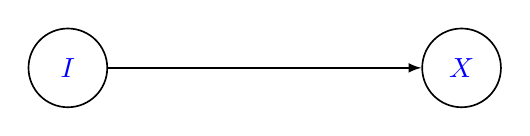
\begin{tikzpicture}[-latex ,auto ,node distance =4 cm and 5cm ,on grid ,
semithick ,
state/.style ={ circle ,top color =white ,
draw , text=blue , minimum width =1 cm}]
\node[state] (A) [left] {$I$};
\node[state] (B) [right = of A] {$X$};
\path (A) edge [] node[above] {} (B);
\end{tikzpicture}
\end{center}

We will partially define the probability distribution with the following structural equation:
\begin{align*}
    X:=I
\end{align*}
Choosing a function that computes $I$ will complete the definition.

Given the dependences indicated, we have as $\mathcal{F}$ the set of constant functions on $\mathcal{I}$. Of these, $I\mapsto0$ minimises $C$.

In this simple case, finding the functional policy reduces to finding the best intervention. 

\subsubsection{Additional dependence}

Let $\mathcal{I},X_1,X_2=\{0,1\}$ and $C(x_1,x_2,I)=x_1$. Suppose $X_2$ is observed before $I$ is computed, so it is a potential input of the policy.

\begin{center}
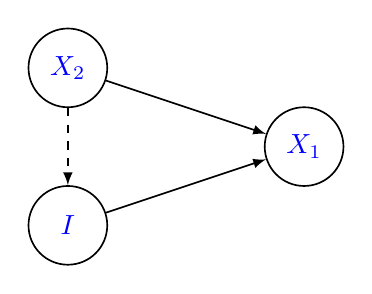
\begin{tikzpicture}[-latex ,auto ,node distance =4 cm and 5cm ,on grid ,
semithick ,
state/.style ={ circle ,top color =white ,
draw , text=blue , minimum width =1 cm}]
\node[state] (B) [right] {$X_1$};
\node[state] (A) [above left = 1cm and 3cm of B] {$X_2$};
\node[state] (C) [below left = 1cm and 3cm of B] {$I$};
\path (A) edge [] node[above] {} (B);
\path (C) edge [] node[above] {} (B);
\draw[dashed] (A) -- (C);
\end{tikzpicture}
\end{center}

We will partially define the distribution with:
\begin{align*}
    X_1 := \mathrm{XOR}(I,X_2)
\end{align*}

We could consider policies that are constant on $\{0,1\}$, or maps $\{0,1\}\to\{0,1\}$. Clearly in this case we want $\Pi:I\mapsto X_2$. If we further knew that $P(X_2=0)=1$, then the constant policy $f:I\mapsto 0$ would perform equally well.

\begin{remark}
The optimal policy isn't straightforward to derive using Causal Bayesian Networks. If we consider the setup above where we are permitted to conduct interventions on the node labeled by $I$, under the standard definition of intervention we would assume that it cuts off any dependence of $I$ on $X_2$. This would limit us to what are here described as constant policies, which are not in general optimal. 

We could address this by proposing that $do()$-interventions could depend on the value of $X_2$ even if $I$ does not depend on it directly. This would invalidate some properties of Causal Bayesian Networks.
\end{remark}

\begin{remark}
If the policy depends on $X_2$, we never need to know the full probability distribution to find the optimal policy.
\end{remark}

\subsubsection{Hidden dependence}
Let $\mathcal{I},X_1,X_2=\{0,1\}$ and $C(x_1,x_2,I)=x_1$. Suppose $X_2$ is not observed.

\begin{center}
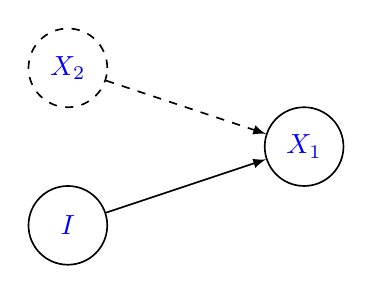
\begin{tikzpicture}[-latex ,auto ,node distance =4 cm and 5cm ,on grid ,
semithick ,
state/.style ={ circle ,top color =white ,
draw , text=blue , minimum width =1 cm}]
\node[state] (B) [right] {$X_1$};
\node[state,dashed] (A) [above left = 1cm and 3cm of B] {$X_2$};
\node[state] (C) [below left = 1cm and 3cm of B] {$I$};
\path (C) edge [] node[above] {} (B);
\draw[dashed] (A) -- (B);
\end{tikzpicture}
\end{center}

We will assume the following structural equations
\begin{align*}
    X_2 &:= \mu_{X_2}\\
    X_1 &:= \mathrm{XOR}(I,X_2)
\end{align*}
Where $\mu_{X_2}\sim \mathrm{Bernoulli}(0.2)$.

In this case, the problem appears to be identical to a problem with the dependence structure of \ref{sssec:simple_case}, and the optimal policy is constant $\Pi:I\mapsto 1$.

\subsubsection{Confounded observations}
Let $\mathcal{I},X_2=\{0,1\}$, $X_1=\{0,1,2\}$ and $C(x_1,x_2,I)=x_1$. Suppose $X_2$ is not observed.

Suppose also that we make infinite observations under some fixed policy $f$, and we are then free to impose our preferred policy $\Pi$.

\begin{center}
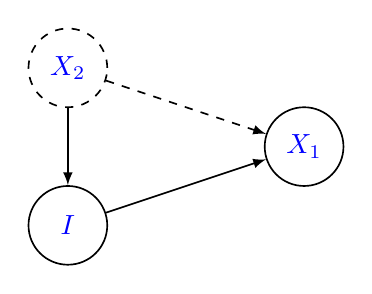
\begin{tikzpicture}[-latex ,auto ,node distance =4 cm and 5cm ,on grid ,
semithick ,
state/.style ={ circle ,top color =white ,
draw , text=blue , minimum width =1 cm}]
\node[state] (B) [right] {$X_1$};
\node[state,dashed] (A) [above left = 1cm and 3cm of B] {$X_2$};
\node[state] (C) [below left = 1cm and 3cm of B] {$I$};
\path (C) edge [] node[above] {} (B);
\draw[dashed] (A) -- (B);
\draw (A) -- (C);
\end{tikzpicture}
\end{center}

We will assume the following structural equations
\begin{align*}
    X_2 &:= \mu_{X_2}\\
    X_1 &:= \neg I + X_2 \\
    f   &:= X_2
\end{align*}
Where $\mu_{X_2}\sim \mathrm{Bernoulli}(0.2)$.

The optimal policy will be $\Pi:I\mapsto 0$, but from our observations it will appear that $X_1 \CI I$ which would suggest that $\Pi$ is no better than the alternative.

\subsubsection{Randomisation}
Let $\mathcal{I}\{0,1\}$, $X_1=\{0,1,2\}$, $N=\{0,1,..,i,..,n\}$ and $C(x_1,i,I)=x_1$. Suppose $X_2$ is not observed.

We wish to estimate the distribution of $X_1$ under fixed policies $f_0:I\mapsto 0$ and $f_1:I\mapsto 1$, and we can sample the system $n$ times. In order to do this, we will in fact be sampling under the policy $r:N\mapsto \{0,1\}$.

\begin{center}
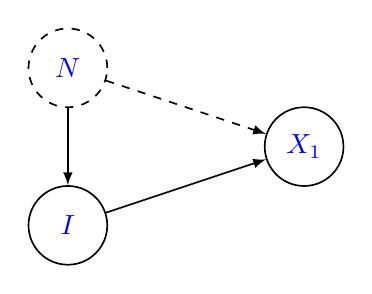
\begin{tikzpicture}[-latex ,auto ,node distance =4 cm and 5cm ,on grid ,
semithick ,
state/.style ={ circle ,top color =white ,
draw , text=blue , minimum width =1 cm}]
\node[state] (B) [right] {$X_1$};
\node[state,dashed] (A) [above left = 1cm and 3cm of B] {$N$};
\node[state] (C) [below left = 1cm and 3cm of B] {$I$};
\path (C) edge [] node[above] {} (B);
\draw[dashed] (A) -- (B);
\draw (A) -- (C);
\end{tikzpicture}
\end{center}

The dependence structure is identical to the previous section, which showed that in general it isn't possible to deduce the optimal policy from these observations. The difference is that we are free to choose $r$.

Suppose there is some set of ``plausible'' functions $\mathcal{H}=\{N\times I\to X_1\}$. If we choose $f'$ such that 
\begin{align}
    \max_{h\in\mathcal{H}} \left| \langle \{h(i,0):r(i)=0\}\rangle - \langle \{h(i,0):i\in\{n\}\} \rangle \right| < \epsilon \label{eq:bin_random}
\end{align}
Where $\langle\cdot\rangle$ denotes an average. If we suppose this also holds for $h(\cdot,1)$, then we can be confident that the subset of samples for which $r(i)=0$ will provide a good estimate for the distribution of $X_1$ under $f_0$, and the subset for which $r(i)=1$ will provide a good estimate for the distribution under $f_1$.




% \subsection{Recovering a model-selection rule}

% Given $f:X\to \mathbb{R}$, define $\text{argmin}_x f(x) = \{x: f(x)\leq f(x')\text{ for all }x'\in X\}$ (this is the standard definition, I just put it here to emphasise that argmin is a set).

% Suppose we have a loss $L_{M^*,C}:\mathcal{M}\to \mathbb{R}$  and a set of models $\mathcal{M}$ with the property that 
% \begin{align}
%     M \in \mathrm{argmin}_M L_{M^*,C}(M)\implies \mathrm{argmin}_I \mathbb{E}_{M(I)}[C(X)] = \mathrm{argmin}_I \mathbb{E}_{M^*(I)}[C(X)] \label{eq:cq_loss1}
% \end{align}
% Then proceed as in Def. \ref{def:causal_query_1} with $D$ replaced by $M^*$.

% Condition \ref{eq:cq_loss1} is too weak - could strengthen it to for every $\epsilon > 0$ there is $\delta > 0$ s.t.
% \begin{align}
%     M \in \{M:L_{M^*,C}(M) < \mathrm{min}_{M'} L_{M^*,C}(M') + \delta \}\implies \mathrm{argmin}_I \mathbb{E}_{M(I)}[C(X)] = \mathrm{argmin}_I \mathbb{E}_{M^*(I)}[C(X)] + \epsilon \label{eq:cq_loss2}
% \end{align}

% Additional complication: given $\mathcal{S}$, we may not be able to find an approximately optimal model $M$. In particular, we may not be able to bound $|L_{M^*,C}(M)-L_{\mathcal{S},C}(M)|$. ($L_{\mathcal{S}}$ needs definition here).

% \textbf{Are there alternative weaker conditions that may be desirable? Do these lead to actually-existing types of causal inference query?}

% It seems like the two things that might be desirable are, informally, policy improvement and sample complexity improvement. 

% \textbf{Weak policy improvement:} given some prior $P_\mathcal{M}$ over $M$ and $P_\mathcal{M'}$ over $M'=\text{argmin}_M L_{\mathcal{S},C}(M)$ and 
% \[I\in \mathrm{argmin}_I \mathbb{E}_{P_{M}}\left[\mathbb{E}_{M^*(I)}[C(X)]\right]\] \[I'\in \mathrm{argmin}_I \mathbb{E}_{P_{M'}}\left[\mathbb{E}_{M(I)}[C(X)]\right]\]
% weak policy improvement:
% \begin{align}
%     \mathbb{E}_{M^*(I')}[C(X)] < \mathbb{E}_{M^*(I)}[C(X)]
% \end{align}
% Note: introducing $P_\mathcal{M}$ and $P_\mathcal{M'}$ suggests replacing the loss $L$ with Bayes rule?

% \textbf{Sample complexity improvement:} suppose we have $L$ such that Eq \ref{eq:cq_loss2} holds, and there exist extra observations $\mathcal{S}_0$ such that for model class $\mathcal{M}$ w.p. $1-\delta$ we have \[|L_{M^*,C}(M)-L_{\mathcal{S}\cup\mathcal{S}_0,C}(M)|<\epsilon\]

% Suppose we have a loss $\tilde{L}_{\mathcal{S},C}$ such that for $\mathcal{M}'=\mathrm{argmin}_M L_{\mathcal{S},C}(M)$ there exist extra observations $\mathcal{S}_0'$ such that $|\mathcal{S}_0'|<|\mathcal{S}_0|$ and
% \[|L_{M^*,C}(M)-L_{\mathcal{S}\cup\mathcal{S}'_0,C}(M)|<\epsilon\]

% ** This needs a universal quantifier.

% \subsection{Inferring a causal model}

% Given data $D$ over variables $\mathbf{V}$, a class of possible causal models $\mathcal{M}$ and a $D$-dependent loss $\mathcal{L}_D:\mathcal{M}\to \mathbb{R}$, which models $M\subset \mathcal{M}$ minimise $\mathcal{L}_D$?

% Examples: Pearl, chapter 2 \cite{pearl_causality:_2009} - uses estimated distribution $\hat{P}$ rather than data $D$. Proposes two algorithms $IC$ and $IC^*$. Both output sets of CBNs with common conditional independence properties.

% $IC$ considers the class $\mathcal{M}\subset\text{CBN}$ which is the union of all causal structures that can be represented as graphs with exactly one node for each $V\in\mathbf{V}$.

% $IC^*$ considers the class that is the union of all causal structures that can be represented as graphs with one node for each $V\in\mathbf{V}$ and one common cause node for each pair of variables.


% \subsection{Predicting the effect of an intervention}

% Given data $D$ over variables $\mathbf{V}$ and intervention space $\mathcal{I}$, outcome variables $\mathbf{Y}\subset\mathbf{V}$ predictor $\hat{M}:\mathcal{I}\to\text{Range}(Y)$ and loss $\mathcal{L}_D:\hat{M}\to\mathbb{R}$, find $\hat{M}$ minimising $\mathcal{L}_D$.*

% What if we want the complete distribution over $Y$ rather than a point estimate?


\section{Key Questions}

\section{Causal Models}

\subsubsection{Definition of Causal Models}

\begin{question}
    Do the major examples of causal models in the literature satisfy Definition \ref{def:causal_models}?
    \begin{itemize}
        \item Causal Bayesian Networks
        \item Structural Causal Models
        \item Potential Outcomes/Rubin Causal Model
        \item Marginal models
    \end{itemize}
\end{question}

\begin{question}
    Are the major examples of causal models in the literature special cases of probability distributions with the "exorcism" assumption (Definition \ref{def:exorcism})?
    \begin{itemize}
        \item Causal Bayesian Networks
        \item Structural Causal Models
        \item Potential Outcomes/Rubin Causal Model
        \item Marginal models
    \end{itemize}
\end{question}

\begin{question}
    Is it possible to use markov kernels rather than policy functions to define policy based causality?
\end{question}

\begin{question}
    Is the exorcism assumption necessary for causal reasoning (Definition \ref{def:exorcism})?
\end{question}

\begin{question}
    What is the appropriate line of reasoning to take if, in Definition \ref{def:exorcism}, we allow $\mathcal{F}\subset A$?
\end{question}

\subsubsection{Relationships between types of causal models}

\begin{question}
    Is there an equivalence between functions with sources of noise for inputs and Markov kernels?
\end{question}

\begin{question}
    One feature of structural causal models is the possibility to derive deterministic maps by substituting constants for the noise variables $u_i$. This could be seen as a generalisation of interventions from operations that replace the right hand side of an assignment with a constant to an operation that makes a more general modification to the right hand side of an assignment.
    
    What is the set of general interventions on an SCM that preserve the Markovian property?
\end{question}

\begin{question}
    What is the precise relationship between the key assumptions in potential outcomes causality (ignorability, common support) and key assumptions identified for policy causality (exorcism, complete interventional projections)?
\end{question}

\subsubsection{Causal models vs probability distributions}

\begin{question}
    Pearl claims there are fundamental differences between causal and probabilistic models \cite{pearl_causality:_2009}. Does policy based causality effectively refute this claim?
\end{question}


\subsubsection{Causal models vs other kinds of models}

\begin{question}
    What is the relationship between general/Markovian causal models and other system models, particularly where interaction with the system is important? 
    
    Relationship could mean: does one type of model a subset of another? Is there some operation that generates one type of model given another?
    \begin{itemize}
        \item First order state space models
        \item Markov Decision Processes
    \end{itemize}
\end{question}

\subsubsection{Weakening causal assumptions}

\begin{question}
    Given a structural causal model, policy based causality doesn't distinguish in type between a policy and a regular node - both are functions of input variable and independent noises. Does this yield a natural spectrum for soft to hard interventions, where soft interventions are "the original function" and hard interventions impose constant functions at the policy node?
\end{question}

\begin{question}
    Given the above spectrum of soft to hard interventions, what options are there for interpolating between these points?
\end{question}

\begin{question}[Intervention cascade]\label{q:intervention_cascade}
    Given the ability to perform a hard intervention on a particular node, does this raise the possibility of performing soft interventions on a number of other nodes?
\end{question}

% \subsubsection{Markovian causal models}

% \begin{question}
%     Is there an appropriate way to define an "approximately Markovian" causal model?
%     Points to consider:
%     \begin{itemize}
%         \item Are there operations we can perform on data generated by a Markovian system that will yield an approximately Markovian system? Example operations: forgetting data for some variables, averaging data over time or over repeated instances.
%         \item Is there a "mathematically neat" way to define approximate Markovianity?
%     \end{itemize}
% \end{question}

\subsection{Causal Inference Problems}

\begin{question}[Generalisation of interventional trials]
    See Question \ref{q:intervention_cascade}.
    
    Motivation: RCTs often estimate the effects of composite interventions in particular contexts, so interpretation is unclear. However, they also reliably identify causal effects, which distinguishes RCT results from any old dataset.
    
    Question: Under what conditions can a *set* of RCT results be generalised? Is there enough causal information in an RCT to permit a "statistical learning theory" type of result for RCT generalisation, or is the problem of generalising RCTs itself limited by nonidentifiability issues?
\end{question}

\begin{question}\label{q:causal_queries}
    What are the key kinds of causal queries? A very preliminary list:
    \begin{itemize}
        \item Control/prediction: how would a system behave if intervention $I$ were applied?
        \item Attribution: what is responsible for the observation of outcome $v$?
        \item Latent variables: identifying latent variables causally responsible for observed data
        \item Causal structure: identifying how observed variables are causally related to one another
    \end{itemize}
\end{question}

\begin{question}
    Detecting latent variables has a clear connection to dimensionality reduction \cite{kummerfeld_causal_2016}. As a general question, how does \emph{causal} latent variable detection differ from other forms of dimension reduction?
    
    As a more specific question, is there a particular form of loss function that is, implicitly or explicitly, assumed in causal latent variable detection? 
\end{question}

\begin{question}\label{q:causal_query_difficulty}
    How should the difficulty of a causal query be measured?
    Some possibilities:
    \begin{itemize}
        \item Observational sample complexity
        \item Interventional sample complexity
    \end{itemize}
\end{question}

\begin{question}
    Is it possible to define a generic set of elements that constitute a causal inference query? For example, a control query might require:
    \begin{itemize}
        \item Outcome/objective
        \item Set of allowed interventions
        \item Set of observations
        \item Hypothesis class
        \item Assumptions
        \item Data
    \end{itemize}
\end{question}

\begin{question}
    Causal queries typically employ assumptions over and above the assumptions made for statistical queries. Are additional assumptions always necessary?
    
    More precisely: given a causal model $M$ for which the class $\mathcal{P}$ of distributions satisfies statistical learnability assumptions (clarification pending), what characterises causal queries that are unresolvable without further assumptions?
\end{question}

\begin{question}\label{q:query_set_of_models}
    Given a causal query (pending definition) and the assumption of a Markovian causal model, does the query induce equivalence classes of causal models? Does this depend on the type of query?
\end{question}

\begin{question}
    Can two identical causal models (Definition \ref{def:causal_models}) with different side information (definition pending) give different answers to a causal query (definition pending)?
\end{question}

\begin{question}
    What are key features in a taxonomy of causal inference problems that aims to group problems by which approaches to solving the problem may/may not work? Do the objects identified in Definition \ref{def:causal_models} - $\mathbf{V}$, $\mathcal{I}$, $\mathcal{P}$ play important roles in such a taxonomy?
\end{question}

\begin{question}
    Given a causal bayesian network $M$ with targets $Y$, other observables $X$ and interventions $\mathcal{I}$ and cost $C:\mathcal{I}\times Y\to\mathbb{R}$, are there control strategies possible with $M$ that may be superior to control strategies possible if only $P(Y|I)$ is known for all $I\in\mathcal{I}$?
\end{question}

\subsection{Causal Discovery}

Causal discovery describes any method of learning a set of Markovian causal models that might describe the causal relationships between variables in a dataset.

\begin{question}
    To what extent have additive noise models been extended to Markov kernels featuring other types of noise? To what extent can they be extended?
\end{question}

\begin{question}
    Is it correct to consider queries about causal structures instrumental queries in service of other aims? Alternatively, should causal structures be added to the list in Question \ref{q:causal_queries}?
\end{question}

Many algorithms for causal structure discovery do not resolve whether $X$ and $Y$ are confounded by an unobserved $Z$ or not. On the other hand, the answer many conceivable causal queries will depend on whether two variables are confounded or directly causally related. The next questions focus on whether structural identification can help with causal queries.

\begin{question}\label{q:discovery_set_of_models}
    A structure discovery algorithm will typically output some class $\mathcal{C}$ of causal models. In some cases these classes are well-defined, for example Markov Equivalence Classes. In some cases it is not so clear - algorithms that cannot detect latent confounders are usually introduced with the assumption that no such confounders exist. However, it is also possible to view them as outputting a large class of causal models that contains many models with latent confounders and some without.
    
    The question here is what classes of causal models are output by the various structure learning algorithms?
\end{question}

\begin{question}
    Considering the model sets in \ref{q:query_set_of_models} and \ref{q:discovery_set_of_models}, when is it possible for the output of a structure discovery algorithm to facilitate answering a causal query - for example, by reducing the query to one that is easier on a metric of difficulty (question \ref{q:causal_query_difficulty}).
\end{question}

\begin{question}
    Which causal discovery algorithms require the assumption of faithfulness?
    \begin{itemize}
        \item PC and IC definitely do
        \item Bayesian score based (e.g. Greedy Equivalence Search) I'm not sure
        \item Additive noise models, information geometric definitely don't
        \item Latent factor detection (BPC, FOFC) - I'm not sure \cite{kummerfeld_causal_2016}
    \end{itemize}
\end{question}

\begin{question}
    What is the relationship between $\lambda$ in $\lambda$-faithfulness and sample complexity of PC-type algorithms?
\end{question}

\begin{question}
    Are there weakenings of faithfulness or $\lambda$-faithfulness, and do these allow for consistency results of their own?
    \begin{itemize}
        \item Some types of faithfulness violations have testable implications, so only some types of faithfulness need to be assumed \cite{ramsey_adjacency-faithfulness_2012}
        \item Some types of faithfulness violations could be benign (e.g. violated faithfulness in $X\to Y$) \cite{peters_structural_2013}
        \item The degree to which faithfulness violations impact the answer to a causal query might scale with the number of "non-transparent" conditional independences 
    \end{itemize}
\end{question}

\begin{question}\label{q:volume_unfaithful}
    Is it possible to lower bound the volume of unfaithful distributions for a set of probability distributions $\mathcal{P}_G$ with parametrisation $\mathbf{a}_G$ that are Markovian to an arbitrary graph $G$? \cite{uhler_geometry_2013}
\end{question}

\begin{question}
    Can entropy-based constraints simplify the analysis of sets of faithful distributions in Question \ref{q:volume_unfaithful} (I don't presently understand what entropy-based constraints are, so this question might make no sense. I just recall a comment that entropy based constraints can be easier to work with than geometry of algebraic varieties).
\end{question}

Both the faithfulness assumption and additive noise model causal discovery identify a "contrast function" $C(P):\mathcal{P}\to\mathbb{R}$ of a probability distribution $P$ that, given a measure $\mu_G$ over $\mathcal{P}$ for each CBN $G$, takes generic values for to some CBNs $\mathcal{G}^*$ and nongeneric values for all others $\mathcal{G}^{*C}$. That is, $\mu_{G^*}(C(P))>0$, and $\mu_{G'}(C(P))=0$ for any $G'\in\mathcal{G}^{*C}$.

\begin{question}\label{q:generalised_genericity}
    These genericity conditions hold for a general class of measures $\mu_G$ - for example, if a distribution $P$ is parametrised by $\{a_i\}$ for a graph $G$, then the genericity conditions might hold for any continuous prior over $\{a_i\}$.
    
    However, to get uniform consistency results, we need to allow for some slack around the value of $C(P)$, and consequently need to shift from "non-transparent" probability distributions having measure 0 under $\mu_G$ to having small measure under $\mu_G$.
    
    For what class of measures can we conclude from $\mu_G(C(P)=c_0)=0$ and $|C(\hat{P})-c_0|<\delta$ that $\mu_G(C(\hat{P})\in B_\delta (c_0)) < \epsilon$? Does this depend strongly on $C$?
    
    $B_\delta(x)$ is a ball of radius $\delta$ around $x$.
\end{question}
    
\begin{question}
    Are there any general properties that contrast functions must satisfy?
\end{question}

\begin{question}
    Is there a method to generate contrasts $C$? See \cite{besserve_group_2017} for a discussion of using group transformations for generating measures $\mu_G$.
\end{question}


\begin{question}
    How to get from Markov kernel composition to random variables to Bayesian networks and back.
\end{question}

\begin{question}
    Relationship between approximate assumptions (exchangeability, stability) and cost minimisability
\end{question}

\begin{question}
    What form do arguments take for approximate assumptions to hold?
\end{question}

\begin{question}
    What do you get if $P(v|i,a,q)=P(v|i,a)$ for one $q\in Q$? (not much? e.g. ``it only works in experiments, but all non-experiments are confounded''
\end{question}

\begin{question}
    If $P(i|a,q)$ has high entropy, does that give any more reason to believe policy exchangeability than if it has low entropy? Consider: high mutual information between $q$ and $v|i,a$, between $v$ and $i$, between $q$ and $i|a$.
\end{question}

\begin{question}
    What is the relationship between strong policy exchangeability $P(v|i,a,q)=P(v|i,a,q')$, even where $\phi(a,q;i)=0$ and structural independence  - $V\CI Q| A,I$ for all $P_H$, $\phi$, $\mu$, $\pi$ and $\theta$?
\end{question}

\begin{question}
    A regular Bayesian net represents independence in a probability distribution. A causal Bayesian net represents an extended notion of independence (e.g. structural independence). 
    
    Proposition: ``extended independence'' must matter because it ultimately cashes out in regular independence. Is this true? Which regular independences do we get from extended independence?
\end{question}

\bibliographystyle{plain}
\bibliography{references.bib}


\end{document}
